\section{Compute et render separation}

Il est proposé une implémentation initiale de MPI en faisant usage de la parallélisation en mémoire partagée, de sorte qu’un nœud soit chargé du rendu et que le calcul s’exécute dans un second processus. Il convient de souligner que la parallélisation du calcul en sous-domaines n’est pas encore proposée ; on parle donc d’un unique processus additionnel.

Dans l’implémentation, exactement 2 rangs MPI sont conservés, l’un pour l’image et l’autre pour le calcul, et les mêmes paramètres de simulation de galaxie que dans le cas de Numba ont été employés. Il a été constaté, dans un premier temps, que MPI répartissait les CPU pour chaque processus MPI de manière équivalente, ce qui faisait que, dans le code, à partir d’un certain nombre de rangs avec Numba, des résultats différents de ceux obtenus avant la séparation apparaissaient, car MPI attribuait le même nombre de CPU au nœud de rendu, qui ne possède pas de parallélisation, et au nœud de calcul, qui, lui, en possède une, ce qui explique le \textit{stalling} à partir de 4 threads. Une modification de l’affinité CPU est alors implémentée dans le contexte de l’exécution ; cette fonction fixe :

\begin{itemize}
    \item le rang 0 au CPU 0,
    \item le rang 1 au reste des CPU 1..15,
\end{itemize}

afin que la répartition ne soit pas effectuée de manière automatique avec \texttt{mpiexec --bind-to none -n 2}. L’option \texttt{--bind-to none} évite qu’OpenMPI impose une liaison automatique qui gênerait l’exécution ; ensuite, le programme lui-même fixe l’affinité correcte avec \texttt{assign\_rank\_affinity}. On obtient alors le résultat attendu, dans lequel l’effet du temps de calcul et de traitement continue de dominer le temps de simulation et, en outre, s’ajoute le fait que, pour cette taille de galaxie, le temps de communication et de synchronisation entre les processus n’est pas très significatif, bien qu’il subsiste la nécessité imminente de pouvoir paralléliser les autres sections de l’algorithme de calcul qui ne sont pas adaptées à la parallélisation avec mémoire partagée, parmi lesquelles le traitement de la grille.

\begin{figure}[htbp]
\centering
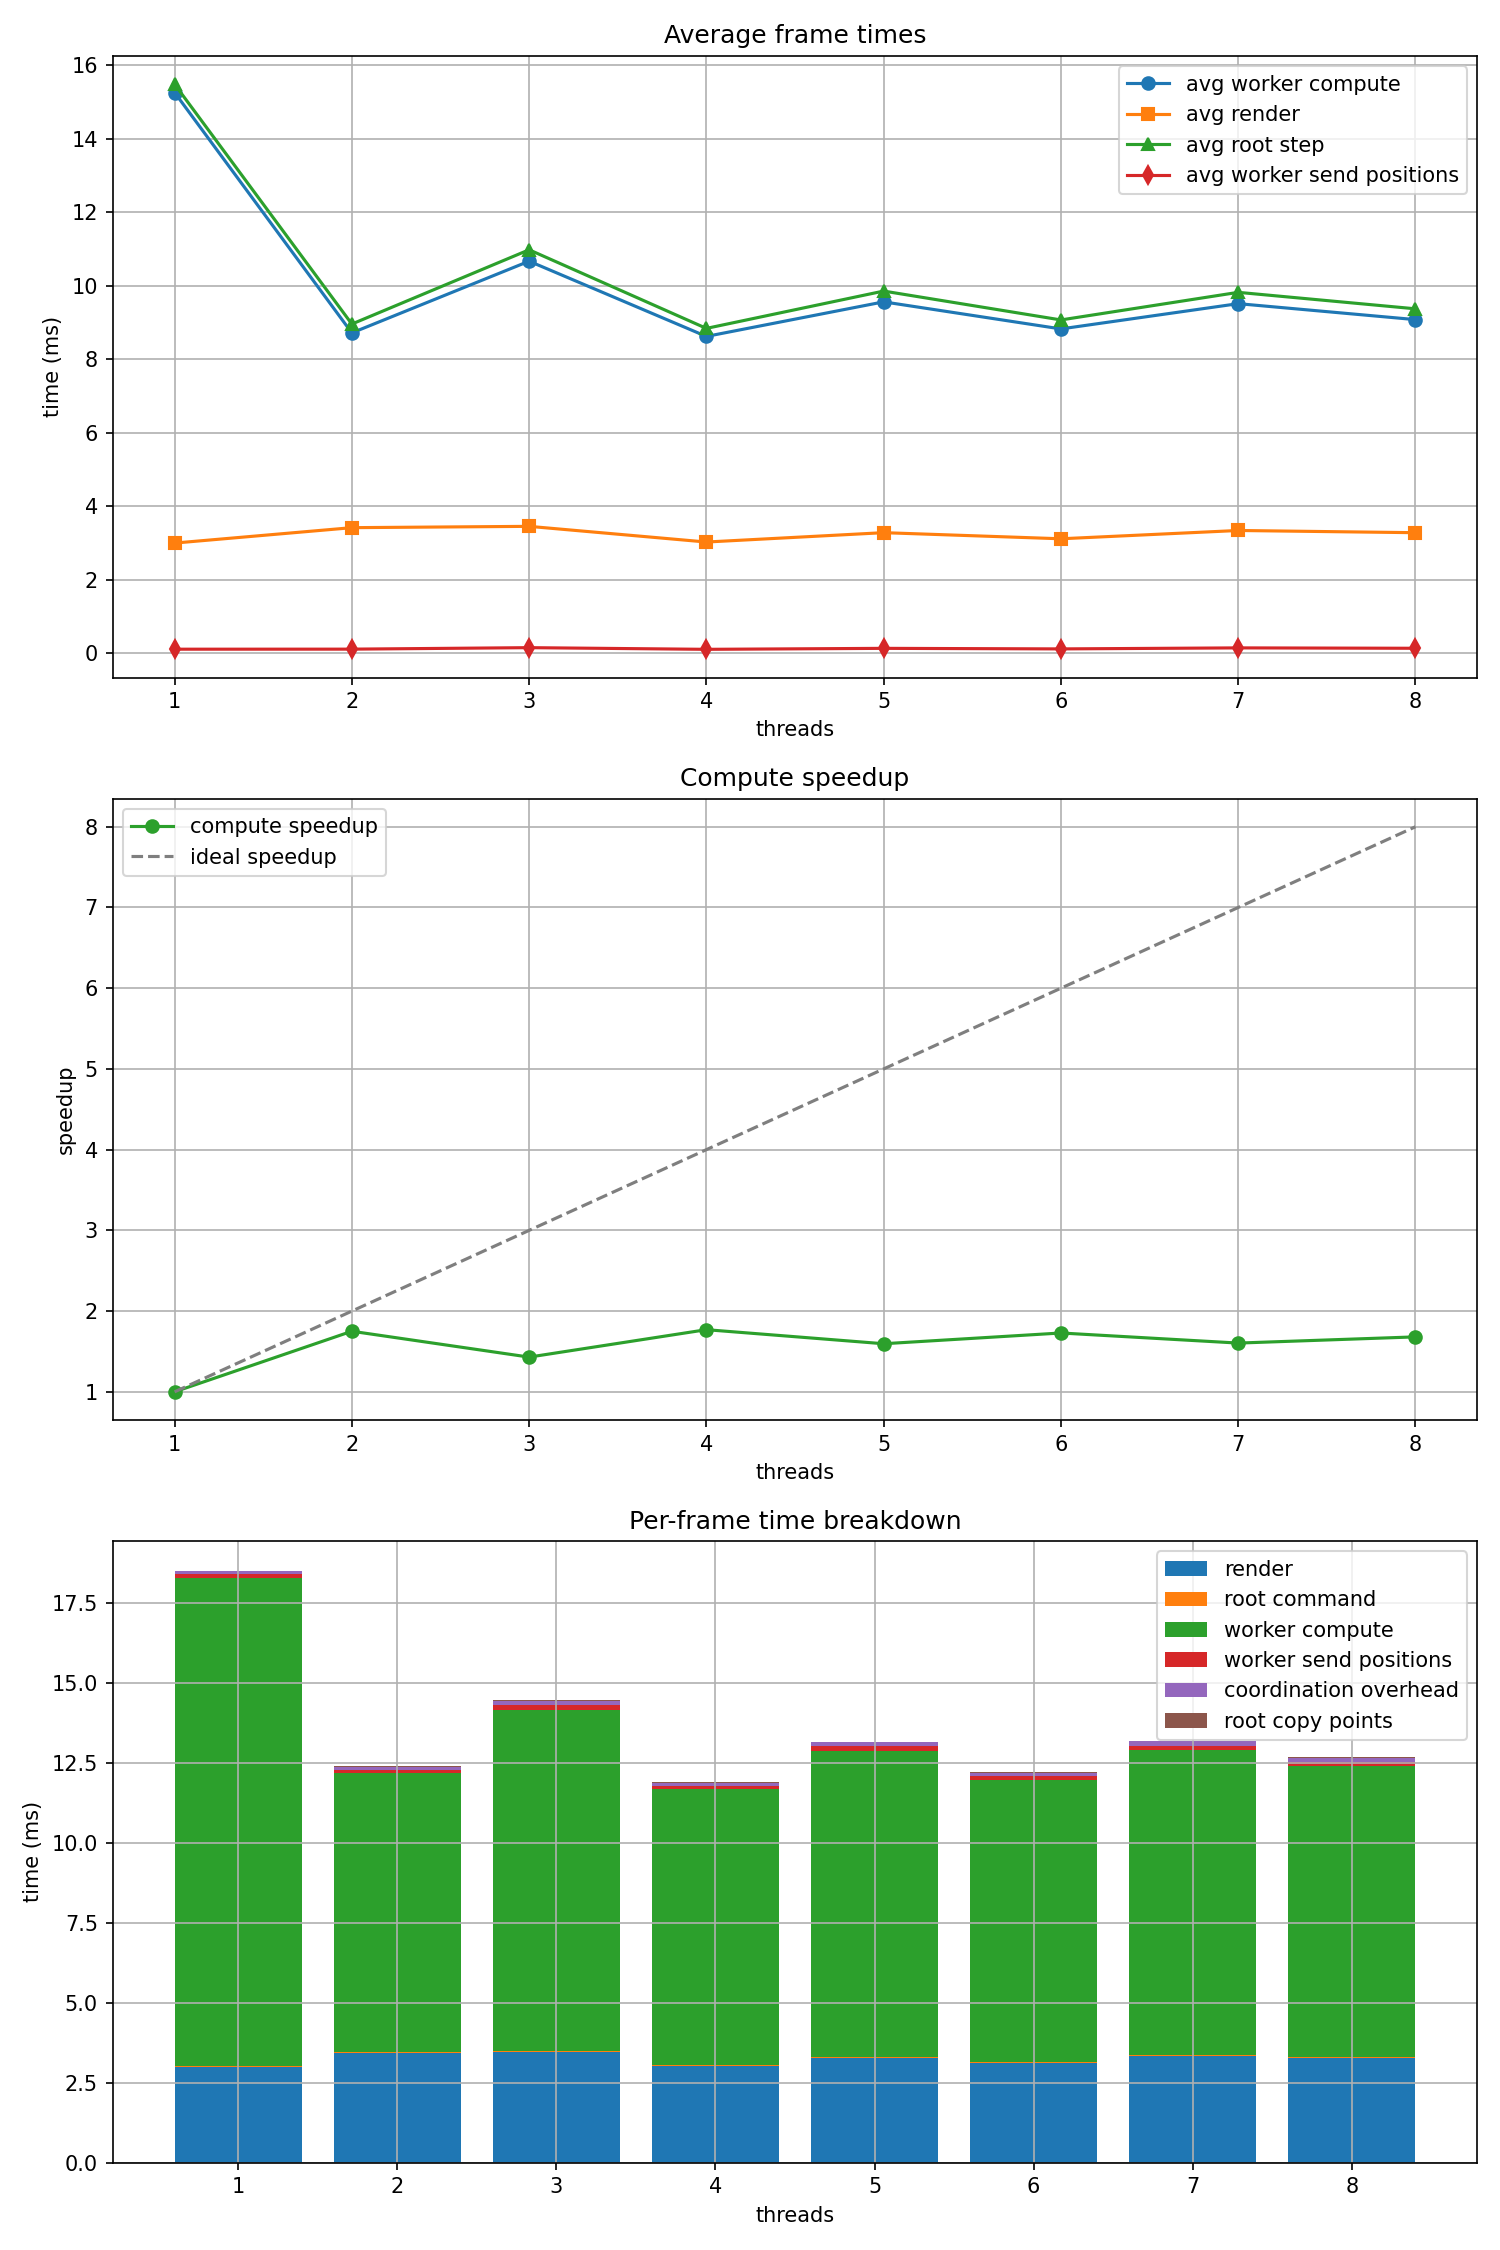
\includegraphics[width=0.82\linewidth]{images/mpi_separation_timings_symetriccpu.png}
\caption{Mesures de la version MPI avec répartition symétrique des CPU entre les deux rangs.}
\label{fig:mpi_separation_timings_symmetric_cpu}
\end{figure}

\begin{figure}[htbp]
\centering
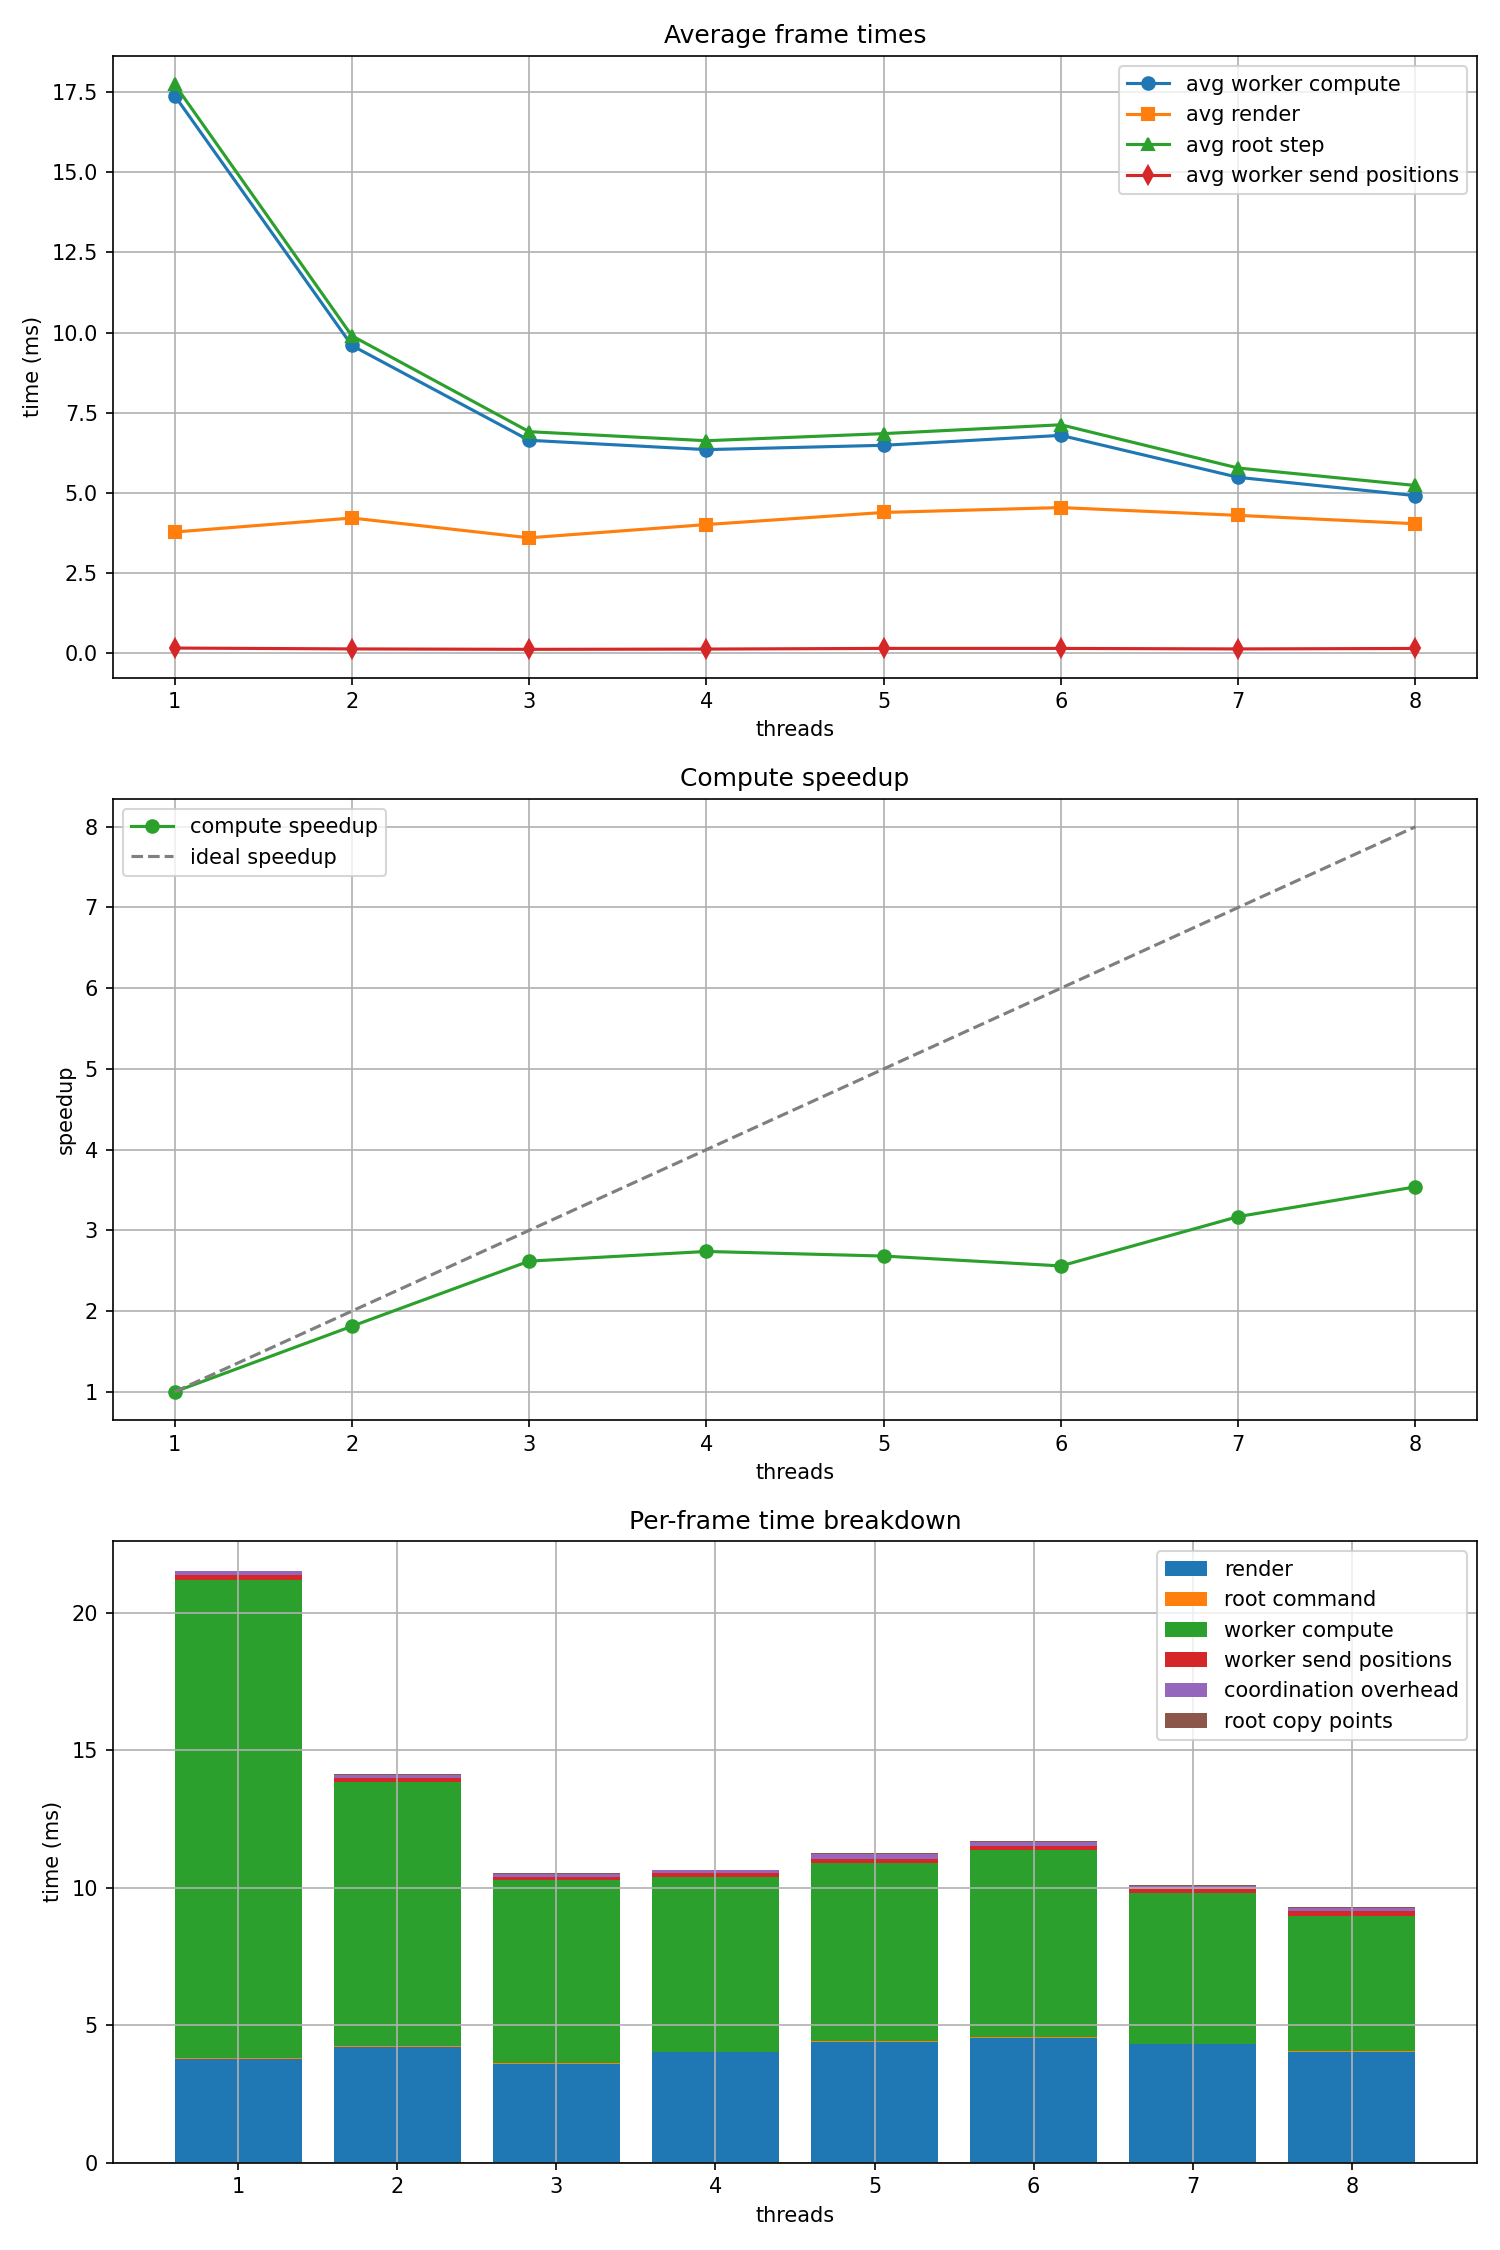
\includegraphics[width=0.82\linewidth]{images/mpi_separation_timings_non_symetriccpu.png}
\caption{Mesures de la version MPI avec affinité CPU non symétrique, où le rang de calcul utilise les CPU restants.}
\label{fig:mpi_separation_timings_non_symmetric_cpu}
\end{figure}
